%	Autor:		Sean Dalton	
%	Datum:		tt.mm.jjjj
%	Short:		Bachelorarbeit
% DOCUMENTCLASS -----------------------------------------------------------------------------------------
\documentclass[12pt,a4paper,oneside,numbers=noenddot,headsepline,captions=tableheading,toc=bibliography,openany]{scrbook}

\usepackage{geometry}
\geometry{a4paper,left=40mm,right=25mm, top=25mm, bottom=25mm, includeheadfoot}


% SPRACHE------------------------------------------------------------------------------------------------
	\usepackage[utf8]{inputenc}
	\usepackage[autostyle,babel,german=guillemets,style=german]{csquotes}
	\usepackage[USenglish,ngerman]{babel} 
	\usepackage{lmodern} %Hochaufloesende Schrift
	\selectlanguage{ngerman}
	

% TABELLEN-----------------------------------------------------------------------------------------------
	\usepackage{multirow} % Tabellen-Zellen �ber mehrere Zeilen1
	\usepackage{multicol} % mehre Spalten auf eine Seite
	\usepackage{tabularx} % F�r Tabellen mit vorgegeben Gr��en
	\usepackage{array}
	\usepackage{float}
	\usepackage{booktabs}
	\usepackage{longtable} % Tabellen �ber mehrere Seiten
	\usepackage{rotating}
	\usepackage[table,xcdraw]{xcolor}
	

	\usepackage{pdflscape}
	
% BILDER-------------------------------------------------------------------------------------------------
	\usepackage{graphicx}
	\usepackage{color}


% ALLGEMEINES--------------------------------------------------------------------------------------------
	\usepackage{amsmath,amssymb} % Mathesachen
	\usepackage[T1]{fontenc} % Ligaturen, richtige Umlaute im PDF
	\usepackage[hyphens,obeyspaces,spaces]{url}		% bricht lange URLs ?sch�n? um
	\usepackage[decimalsymbol=comma]{siunitx}
	\usepackage[onehalfspacing]{setspace}
	\setlength{\parindent}{0cm}	% Disable automatic parindent
	\usepackage{placeins}
	\sloppy
	
	\usepackage{pdfpages}
	\usepackage{enumitem}
	\graphicspath{{_img/}}
% PDF-----------------------------------------------------------------------------------------------------
	\usepackage{pdfpages}
	\usepackage[ngerman,%
	pdfauthor={Sean Dalton},%
	pdftitle={Entwicklung der eingebetteten Hardware einer modularen Antriebsplattform},%
	colorlinks=true,linkcolor=black,citecolor=black,filecolor=black,urlcolor=black%
	]{hyperref}

% ABKÜRZUNGEN --------------------------------------------------------------------------------------------
	\usepackage[nohyperlinks]{acronym}


% BIBLATEX -----------------------------------------------------------------------------------------------
	\usepackage[backend=bibtex,%
	style=IEEEtran,%
	bibstyle=numeric,%
	citestyle=numeric,%
	sorting=none,%
	]{biblatex}
	\bibliography{_bib/biblio}
	
% QUELLCODE -------------------------------------------------------------------
\usepackage{listings}
\definecolor{mygreen}{RGB}{28,172,0} 		% color values Red, Green, Blue
\definecolor{mylilas}{RGB}{170,55,241}
\lstset{language=Matlab,%
	basicstyle=\footnotesize\ttfamily,
	breaklines=true,%
	morekeywords={matlab2tikz},
	keywordstyle=\color{blue},%
	morekeywords=[2]{1}, keywordstyle=[2]{\color{black}},
	identifierstyle=\color{black},%
	stringstyle=\color{mylilas},
	commentstyle=\color{mygreen},%
	showstringspaces=false,%without this there will be a symbol in the places where there is a space
	numbers=left,%
	numberstyle={\tiny \color{black}},% size of the numbers
	numbersep=9pt, % this defines how far the numbers are from the text
	emph=[1]{for,end,break},emphstyle=[1]\color{red}, %some words to emphasise
	%emph=[2]{word1,word2}, emphstyle=[2]{style},    
}	
	
% DOCUMENT ------------------------------------------------------------------------------------------------
\begin{document}

%\pagestyle{empty}


\cleardoublepage

% ----------------------------------------------------------------------------------------------------------
% TITELSEITE -----------------------------------------------------------------------------------------------
% ----------------------------------------------------------------------------------------------------------
\begin{titlepage}
	\singlespacing
	
%----------------Einzelnes Logo	
	\begin{center}
		
\includegraphics[width=0.5\textwidth]{logo}
	\end{center}

%----------------Zwei Logo		
%	\begin{figure}
%		\centering
%		\begin{minipage}[b]{0.5\textwidth}
%			
\includegraphics[width=\textwidth]{_img/Logo_Smart_RGB}
%		\end{minipage}
%		\hfill
%		\begin{minipage}[b]{0.4\textwidth}
%			
\includegraphics[width=\textwidth]{_img/logo}
%		\end{minipage}
%	\end{figure}
	
	\begin{center}
		\vspace*{3cm}
		\Huge
		\textbf{Entwicklungsprojekt}\\
		\vspace*{0.5cm}
		\large
		zur Erlangung des akademischen Grades\\
		Bachelor of Engineering (B.Eng.)\\
		\vspace*{1cm}
		\huge
		\textbf{Entwicklung der eingebetteten Hardware einer modularen Antriebsplattform }\\
		\vspace*{2cm}
		\vfill
		\normalsize
		\newcolumntype{x}[1]{>{\raggedleft\arraybackslash\hspace{0pt}}p{#1}}
		
		\begin{tabular}{x{6cm}p{7.5cm}}
			\rule{0mm}{5ex}\textbf{Autor:} & Sean William Dalton\newline sean.dalton@hs-bochum.de\newline Matrikelnummer: 013208208\\
			\rule{0mm}{5ex}\textbf{Erstgutachter:} & Prof.\ Dr.-Ing.\ Arno Bergmann \\
			\rule{0mm}{2ex}\textbf{Zweitgutachter:} &  \\ 
			\rule{0mm}{5ex}\textbf{Abgabedatum:} & tt.mm.jjjj\\ 
		\end{tabular} 
	\end{center}
\end{titlepage}
\onehalfspacing
\cleardoublepage
%\section*{Eidesstattliche Erklärung}
\thispagestyle{empty}

\begin{verbatim}

\end{verbatim}

\begin{Large}
	
	Eidesstattliche Erklärung zur Abschlussarbeit:
	
	\enquote{Entwicklung der eingebetteten Hardware einer modularen Antriebsplattform}
	
\end{Large}

\begin{verbatim}


\end{verbatim}
Ich versichere, die von mir vorgelegte Arbeit selbstständig verfasst zu haben. Alle Stellen, die wörtlich oder sinngemäß aus veröffentlichten oder nicht veröffentlichten Arbeiten anderer entnommen sind, habe ich als entnommen kenntlich gemacht. Sämtliche Quellen und Hilfsmittel, die ich für die Arbeit benutzt habe, sind angegeben. Die Arbeit hat mit gleichem Inhalt bzw. in wesentlichen Teilen noch keiner anderen Prüfungsbehörde vorgelegen.



\begin{displaymath}
% use packages: array
\begin{array}{ll}
Unterschrift:~~~~~~~~~~~~~~~~~~~~~~~~~~~~~~~~~~~~~~~~~~
& Ort, Datum:~~~~~~~~~~~~~~~~~~~~~~~~~~~~~~~~~~~~~~~~~~
\end{array}
\end{displaymath}

\cleardoublepage
% ----------------------------------------------------------------------------------------------------------
% VERZEICHNISSE --------------------------------------------------------------------------------------------
% ----------------------------------------------------------------------------------------------------------
 \pagenumbering{roman}
 
 \tableofcontents
 \addcontentsline{toc}{chapter}{Inhaltsverzeichnis}
 \cleardoublepage

\chapter*{Abkürzungsverzeichnis}
\addcontentsline{toc}{chapter}{Abkürzungsverzeichnis}
\begin{acronym}[PMSM]	% längste Abkürzung
	\acro{ASM}{Asynchronmaschine}
	\acro{GSM}{Gleichstrommaschine}
	\acro{PMSM}{Permanentmagneterregte Synchronmaschine}	
\end{acronym}
\cleardoublepage

\pagestyle{plain}

\chapter*{Symbolverzeichnis}
\addcontentsline{toc}{chapter}{Symbolverzeichnis}

\begin{longtable}{p{3cm}p{8cm}p{2cm}}
	\setlength\tabcolsep{9pt}
Symbol & Bedeutung                & Einheit               \\ \hline
	\endfirsthead
Symbol             & Bedeutung                & Einheit               \\ \hline
	\endhead
	\toprule
	$B$			& magnetische Flussdichte				& \si{\tesla} \\
	$D$			& Elektrische Flussdichte				& \si{\ampere\second\per\square\meter} \\
$E$			& Elektrische Feldstärke				& \si{\volt\per\meter} \\
$H$			& magnetische Feldstärke				& \si{\ampere\per\meter} \\

\bottomrule
\end{longtable}


\cleardoublepage
\pagestyle{headings}
\pagenumbering{arabic}
\setlength{\parskip}{0.1em}
% ----------------------------------------------------------------------------------------------------------
% INHALT ---------------------------------------------------------------------------------------------------
% ----------------------------------------------------------------------------------------------------------

% -*- coding: utf-8 -*-
% !TEX encoding = UTF-8 Unicode
% !TEX root =  main.tex

\chapter{Beispiel Kapitel}
\label{chap:beispiel-kapitel}

In diesem Kapitel wird eine sehr kurze Einleitung in die Verwendung von \verb|LaTeX| beschrieben.\\
Für die Erstellung der Arbeit kann über \url{http://www.texstudio.org/} mit installierter TeX-Distribution \url{https://miktex.org/} das TeXstudio heruntergeladen werden. 

\section{Abbildungen}
Eine Abbildung lässt sich einfach über einfügen: \par\medskip

\lstset{language=TeX}
\begin{lstlisting}
\begin{figure}[h]
\centering
\includegraphics[width=\textwidth]{foc-ac-dc.pdf}
\caption{Beschriftung der Abbildung}
\label{fig:foc-ac-dc}
\end{figure}
\FloatBarrier
\end{lstlisting}

Die breite der Abbildung kann einerseits skaliert oder direkt im Maßstab von \SI{14.5}{\centi\meter} erstellt werden.
Wenn die Abbildung maßstabsgetreu erstellt wird, muss \verb|\centering| und der optionale Befehl \verb|[width=\textwidth]| nicht zwingend übernommen werden.\par\medskip

Es werden beim Auftreten des Befehls \verb|\FloatBarrier| alle bis dahin eingefügten Float-Umgebungen gesetzt Das kann z.B. dazu verwendet werden, dass Floats, wie figure oder table, nicht unterhalb einer neuen \verb|section| oder \verb|chapter| ausgegeben werden.\par\medskip

Abbildung \ref{fig:foc-dc-ac} zeigt \ldots \par\medskip

\begin{figure}[h]
	\centering
	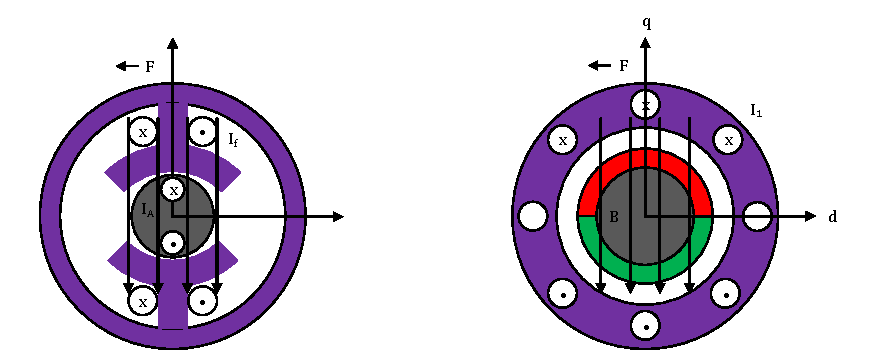
\includegraphics[width=\textwidth]{foc-dc-ac.pdf}
	\caption{Beschriftung der Abbildung}
	\label{fig:foc-dc-ac}
\end{figure}
\FloatBarrier

Durch setzten des \verb|[h]| hinter der \verb|figure| Umgebung, kann die Positionierung der Abbildung festgelegt werden.\par\medskip

Dabei sind folgende Werte ebenfalls möglich:

\begin{enumerate}
	\item h (here) - Gleicher Ort
	\item t (top) - Oben auf der Seite
	\item b (bottom) - Unten auf der Seite
	\item p (page) - Auf einer eigenen Seite
	\item ! (override) - Erzwingt die angegebene Position
\end{enumerate}

\section{Tabellen}\label{sec:tab}

Zur Erstellung einfacher Tabellen, bietet die Website \url{http://www.tablesgenerator.com/} eine einfach zu bedienende Oberfläche. \par\medskip %erzeugt einen mittleren Abstand

Für komplexere Tabellen können die \verb|multicol| und \verb|multirow| Pakete verwendet werden, wie in Tabelle \ref{tab:vgl_mosfet} dargestellt \cite{dalton}.
\begin{table}[h]
		\centering
	\renewcommand{\arraystretch}{1.6}
\begin{tabular}{lc|c|c|c|l}
	\cline{3-5}
	& \multicolumn{1}{l|}{} & \multicolumn{3}{c|}{MOSFET}             &  \\ \cline{3-5}
	& \multicolumn{1}{l|}{} & IRFS7530       & IPB019N08N3 & CSD19536KCS &  \\ \cline{3-5}
	& \multicolumn{1}{l|}{} & International Rectifier       & Infineon & Texas Instruments &  \\ \cline{1-5}
	
	\multicolumn{1}{|l|}{\multirow{4}{*}{\begin{turn}{90}Parameter\end{turn}}} & $Q_{\mathsf{G}}$                    &   354 \nano\coulomb             &  206 \nano\coulomb           &   153 \nano\coulomb      &  \\ \cline{2-5}
	\multicolumn{1}{|l|}{}                                                           & $Q_{\mathsf{GS}}$                   &  62 \nano\coulomb             &  50 \nano\coulomb          &  37 \nano\coulomb       &  \\ \cline{2-5}
	\multicolumn{1}{|l|}{}                                                           & $Q_{\mathsf{GD}}$                   & 73 \nano\coulomb              &  30 \nano\coulomb           &  17 \nano\coulomb       &  \\ \cline{2-5}
	\multicolumn{1}{|l|}{}                                                           & $R_{\mathsf{DSon}}$                 & 1,4 \milli\ohm & 1,9 \milli\ohm            &  3,5 \milli\ohm        &  \\ \cline{1-5}
\end{tabular}
	
	\caption{Vergleich verschiedener MOSFET \cite{dalton}}
	\label{tab:vgl_mosfet}
\end{table}
\FloatBarrier

\section{Zitate}\label{sec:cite}
Für Zitationen wird \verb|BibLaTeX| verwendet. Als Backend wird \verb|bibtex| vom Compiler verlangt.


\begin{quote}
\enquote{Bei jeder permanentmagneterregten Synchronmaschine ändern sich die Induktivitäten in Abhängigkeit von der Last. In erster Linie sind dafür die Sättigungseffekte, aber auch die Kreuzkopplung verantwortlich.} \autocite[S.~2]{ternes2015}
\end{quote}

Im Text zitierte Werke werden über die Syntax \verb|\textcite[S.~2]{ternes2015}| korrekt zitiert. Beispielsweise: Wie in \cite{ternes2015} erläutert, sind die Induktivitäten abhängig von der Last \ldots   \par\medskip

Der aktuelle Stil des Literaturverzeichnisses und der Zitationen ist \verb|IEEEtran|, kann aber auch in Absprache geändert werden, dazu empfiehlt es sich, die \verb|BibLaTeX|-Dokumentation zu konsultieren.\\
\clearpage
\section{Anhänge}\label{sec:Anhang}
Um Anhänge zu referenzieren, können diese mit Hilfe des  erstellten Anhangs (vgl. \ref{anhang_LastenheftEpOS}) referenziert werden.

\section{Formeln}\label{sec:Formeln}

Bei Implementierung von Formeln mit eingesetzten Werten, erweist sich eine Kombination von Tabelle und Formel als Sinnvoll. Tabelle \ref{tab:param_voltageDrop} zeigt die in Formel \ref{eq:voltagedrop} eingesetzten Parameter, mit Beschreibung sowie dem zugehörigen Wert \cite{drv8303}. \par\medskip

\begin{table}[h]
	\centering
	\begin{tabular}{ccc}
		\hline
		Parameter        &       Beschreibung        &           Wert           \\ \hline
		$V_{\mathsf{0}}$    & Maximale Ausgangsspannung &        3,3\ \volt        \\
		$V_{\mathsf{REF}}$   &     Referenz-Spannung     &        3,3\ \volt        \\
		$G$           &    Verstärkungsfaktor     & 40 $\frac{\volt}{\volt}$ \\
		${R}_{\mathsf{SHUNT}}$ &     Shunt-Widerstand      &    $500\ \micro\ohm$     \\ \hline
	\end{tabular}
	\caption{Parameter der Operationsverstärker-Einstellungen des DRV8303}
	\label{tab:param_voltageDrop}
\end{table}


\begin{equation}
\centering
V_{\mathsf{Smax}} = {\lvert ({SN}_{\mathsf{x}} - {SP}_{\mathsf{x}}) \rvert}_{\mathsf{max}} = \left( \frac{ \left({V}_{0} - \frac{ {V}_{\mathsf{REF}}}{2} \right)}{G}\right)   = 41,25\ \milli \volt
\label{eq:voltagedrop}
\end{equation}
\FloatBarrier

%%% Local Variables: 
%%% mode: latex
%%% TeX-master: "main"
%%% TeX-open-quote: "\\enquote{"
%%% TeX-close-quote: "}"
%%% LaTeX-csquotes-open-quote: "\\enquote{"
%%% LaTeX-csquotes-close-quote: "}"
%%% End: 

%\input{_content/einleitung}
%\input{_content/grundlagen}
%\input{_content/systemkonzipierung}
%\input{_content/implementierung}
%\input{_content/verifikation}
%\input{_content/fazit}
\clearpage

   
%Almost done
\pagenumbering{Roman}
\clearpage

% ----------------------------------------------------------------------------------------------------------
% REFERENZEN -----------------------------------------------------------------------------------------------
% ----------------------------------------------------------------------------------------------------------
\listoffigures
\addcontentsline{toc}{chapter}{Abbildungsverzeichnis}
\clearpage

\listoftables
\addcontentsline{toc}{chapter}{Tabellenverzeichnis}
\clearpage

%\printbibliography
\clearpage


%Ende der Arbeit -----------------------------------------------------------------------
\end{document}